Si precisa che tutti in tutti gli scenari simulati si assume che la rete sia completamente connessa per cui da un qualsiasi nodo \textit{x} è possibile raggiungere tramite 1 o più nodi il nodo \textit{sink}.
\\\\
\textit{1) TX Time}: come mostrato in \textbf{Figura \ref{fig:TXTime_final}}, la versione che racchiude tutte le modifiche si comporta meglio rispetto alle altre soluzioni. Ovviamente in questo caso non solo si riduce di molto il numero di wake-up message scambiati durante la fase di relay selection, ma vengono meno tutti i wake-up message usati per sollecitare il nodo sender prima che i receiver inviino il pacchetto CTS.\\
Anche qui il coefficiente di miglioramento aumenta all'aumentare del numero di pacchetti DATA generata dai nodi della rete.\\
In particolare i miglioramenti sono del 77-80\% rispetto la versione base del protocollo GreenWUP e del 20-35\% rispetto ala variante con Auto-WakeUp.
\\\\
\textit{2) Energy Consuption}: come mostrato in \textbf{Figura \ref{fig:EnergySpent_final}}, c'è un piccolo miglioramento anche a livello di energia complessiva consumata dai nodi della rete. Ovviamente questo risultato era aspettato in quanto qui si sommano i vantaggi delle varianti di Relay-Selection e Auto-WakeUp in termini di invio di pacchetti (che siano questi di wake-up o RTS/CTS). Si ha infatti un piccolo miglioramento del 2-4\% rispetto la variante con Relay-Caching e un miglioramento totale di circa 15-18\% rispetto la versione base di GreenWUP.
\\\\
\textit{3) End-to-End Latency}: come mostrato in \textbf{Figura \ref{fig:Latency_final}}, nel caso della latenza quest'ultima variante si comporta praticamente come la versione con Relay-Caching tranne per qualche piccolo peggioramento in alcuni casi. \\
In particolare si ha un piccolo peggioramento che varia tra lo 0.5-1\% rispetto la versione con Relay-Caching mentre si ha un miglioramento del 20-26\% rispetto la versione base del protocollo GreenWUP. 
\\\\
\textit{4) Packet Delivery Ratio}: come mostrato in \textbf{Figura \ref{fig:PDR_final}}, vale quanto detto per la latenza end-to-end. Quest'ultima variante si comporta allo stesso modo della versione con Relay-Caching, presentando, di fatto, un piccolo peggioramento rispetto la versione base del protocollo GreenWUP base.\\
In particolare si ha un peggioramento dello 0.2\%, un peggioramento che non comporta grossi problemi, infatti, come tutte le altre varianti proposte, quest'ultima garantisce in media la carretta ricezione del 99.8\%.

\begin{figure}[H]
  \begin{subfigure}[t]{0.49\linewidth}
    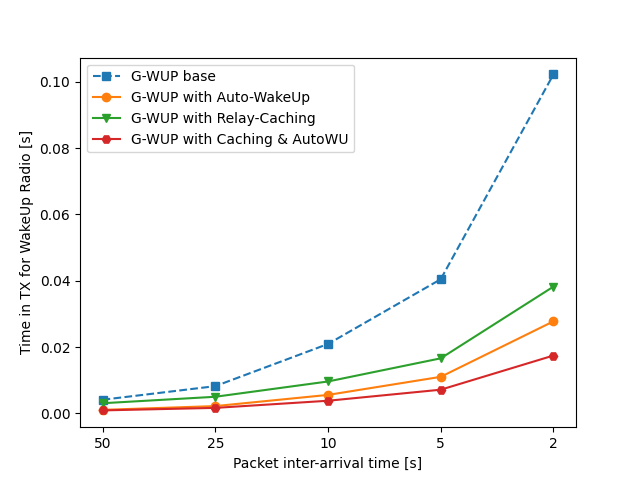
\includegraphics[width=1.1\linewidth]{Contents/Images/graphs/final/tx_time.png}
    \caption{TX Time for the WUR}
    \label{fig:TXTime_final}
  \end{subfigure}
  \begin{subfigure}[t]{0.49\linewidth}
    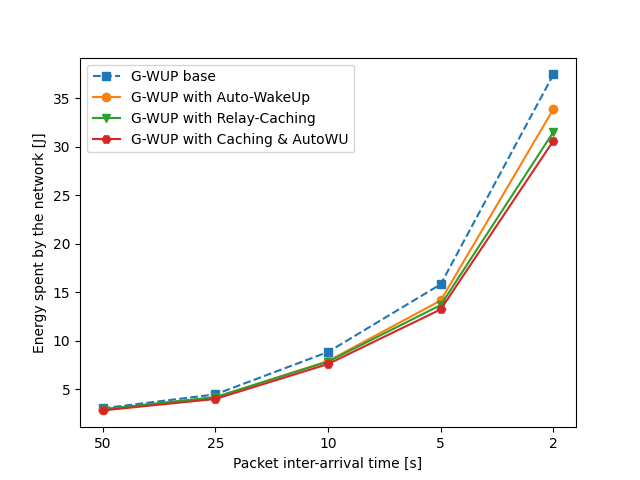
\includegraphics[width=1.1\linewidth]{Contents/Images/graphs/final/energySpent.png}
    \caption{Energy Consuption}
    \label{fig:EnergySpent_final}
  \end{subfigure}
  \begin{subfigure}[t]{0.49\linewidth}
    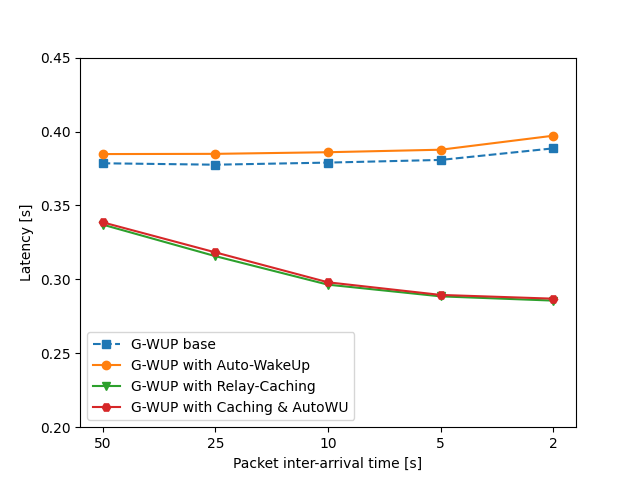
\includegraphics[width=1.1\linewidth]{Contents/Images/graphs/final/latency.png}
    \caption{End-to-End Latency}
    \label{fig:Latency_final}
  \end{subfigure}
  \begin{subfigure}[t]{0.49\linewidth}
    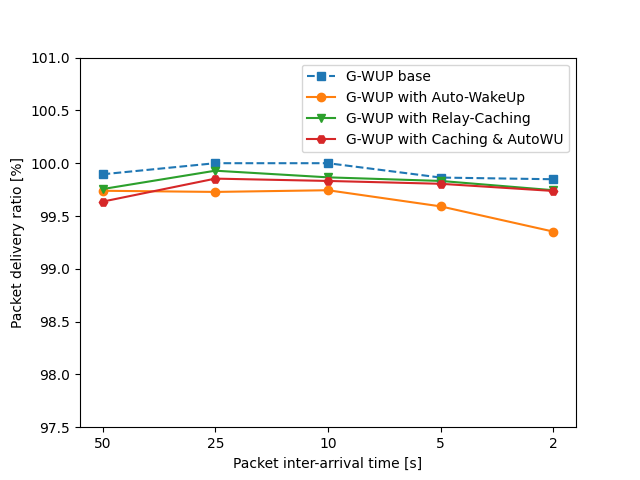
\includegraphics[width=1.1\linewidth]{Contents/Images/graphs/final/pdr.png}
    \caption{Packet Delivery Ratio}
    \label{fig:PDR_final}
  \end{subfigure}
  \caption{Confronto delle prestazioni tra versione base di GreenWUP (blu) e le varianti proposte}
  \label{fig:final}
\end{figure}

La versione All-in-One è quindi efficace nel ridurre la latenza e il consumo energetico di GreenWUP, ad un prezzo di un leggero degrado delle prestazioni in termini di packet delivery ratio.